\ifx\wholebook\relax \else

\documentclass[b5paper]{article}
\usepackage[nomarginpar
  %, margin=.5in
]{geometry}

\addtolength{\oddsidemargin}{-0.05in}
\addtolength{\evensidemargin}{-0.05in}
\addtolength{\textwidth}{0.1in}

\usepackage[en]{../prelude}

\setcounter{page}{1}

\begin{document}

\title{Numerals}

\author{Xinyu LIU
\thanks{{\bfseries Xinyu LIU} \newline
  Email: liuxinyu99@hotmail.com \newline}
  }

\maketitle
\fi

\markboth{Numerals}{A tour of numbers}

\ifx\wholebook\relax
\chapter{Numerals}
\fi

\epigraph{The total number of minds in the universe is one.}{Erwin Schrödinger}

Numbers appear everywhere in our life. For example, this news: \enquote{\textit{The 2024 Paris Olympic Games to an end on Sunday August 11, 2024. Paris is the second city, after London, to host the Summer Olympics three times. It set a record of gender equality, with 5,250 male and 5250 female athletes. In total, 32 sports and 329 events were featured, with 206 countries and regions participating. Four new sports made their debut: skateboarding, surfing, sport climbing, and breakdancing. A total of 329 gold medals were up for grabs. Athletes from various countries and regions demonstrated outstanding athleticism. The United States and China tied for the most gold medals, with each securing 40. The United States also led in silver medals with 44 and bronze medals with 42.}} It contains 14 numbers among the total of 120 words. We don't know who invented the numerals because they show up in almost all historic documents to the very early time. Some believe numerals arose with language. Anthropologists identified numbers inscribed in bones, stones, caves, clay, etc. We can also find such clues in our languages, for example in English, eleven comes from `endleofan', meaning (ten) left one; twelve comes from `twelf', meaning left two.

\section{Rosetta stone}
\index{Rosetta stone}  \label{sec:rosetta-stone}

\begin{figure}[htbp]
 \centering
 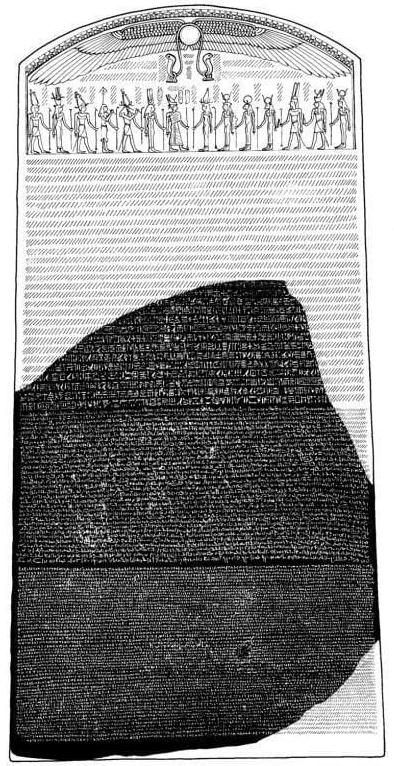
\includegraphics[scale=0.5]{img/Rosetta-stone-recons}
 \caption{Rosetta stone is broken in the middle.}
 \label{fig:rosetta-stone-recons}
\end{figure}

There is a famous object in room 4 of the British museum, the Rosetta stone. It's a broken inscribed stela with the length of 112cm, the width of 76cm (figure \ref{fig:rosetta-stone-recons}). One can identifies some Greek characters like \cref{fig:rosetta-greek} (see \cref{tab:greek-alphabet} of Greek alphabet) in the bottom, while the remaining are mystery ancient characters. When read carefully, there are two different types: a curved form as in \cref{fig:rosetta-demotic} in the middle of the stone, and some small pictures as in \cref{fig:rosetta-hieroglyphs} on the top.

\begin{figure}[htbp]
  \centering
  \subcaptionbox{54 lines in Ancient Greek.\label{fig:rosetta-greek}}{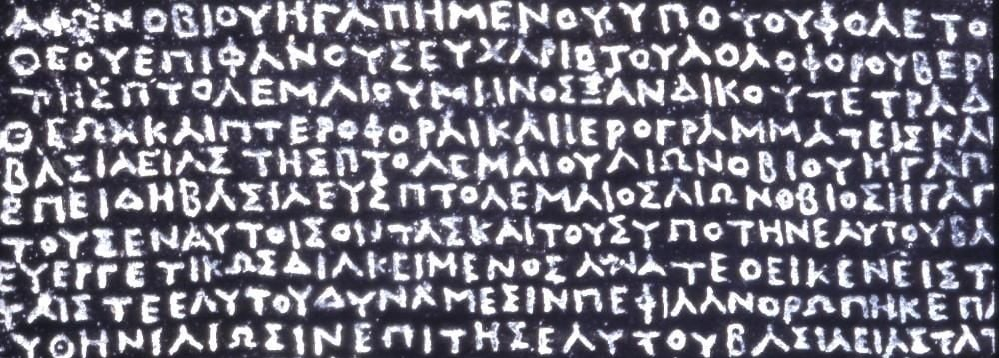
\includegraphics[scale=0.5]{img/Rosetta-Greek}} \\
  \subcaptionbox{32 lines in Demotic, a cursive form of Hieroglyphics use for ordinary document.\label{fig:rosetta-demotic}}{\quad 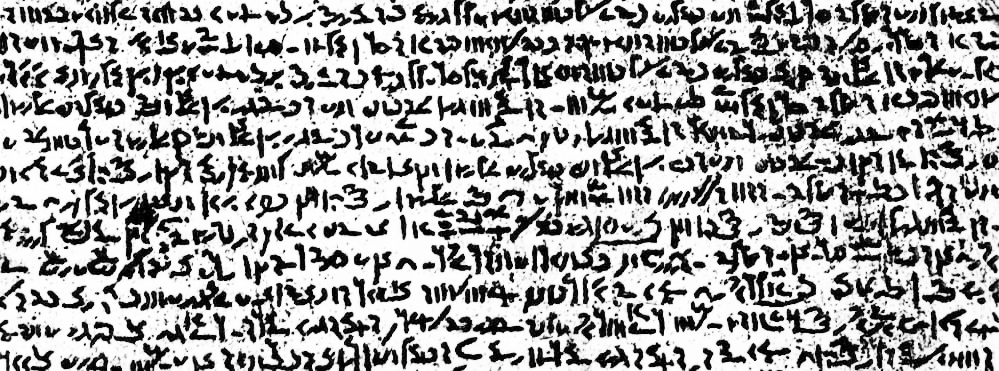
\includegraphics[scale=0.5]{img/Rosetta-Demotic}\quad} \\
  \subcaptionbox{14 lines in Hieroglyphic, the script most used for religious texts.\label{fig:rosetta-hieroglyphs}}{\qquad 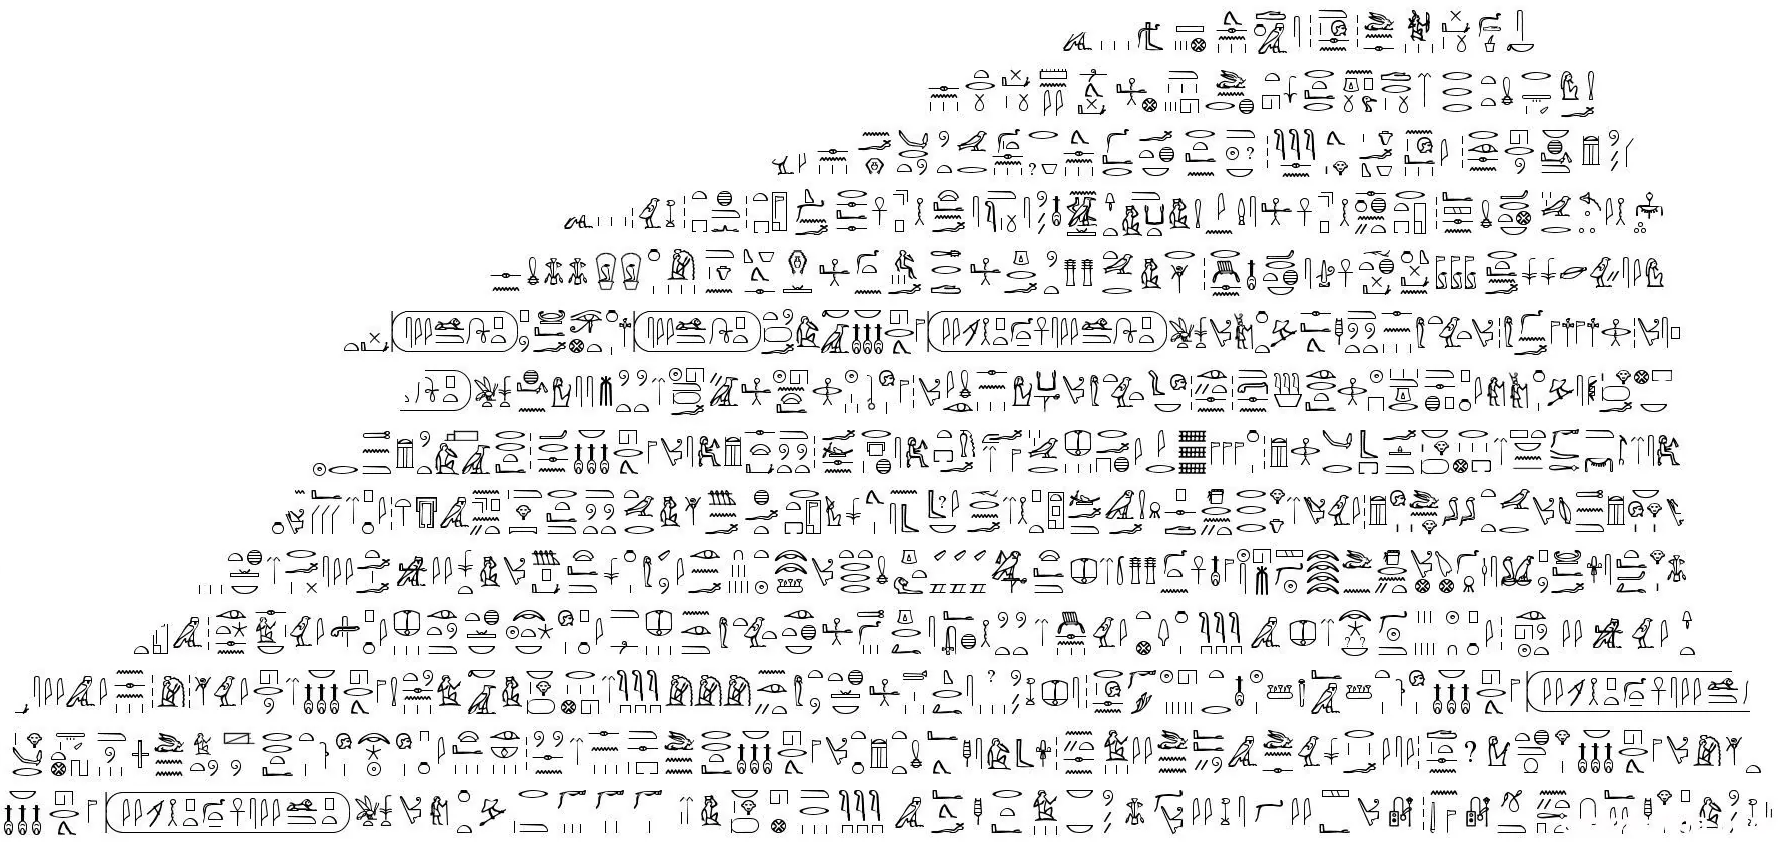
\includegraphics[scale=0.3]{img/Rosetta-Hieroglyphs-c}\qquad}
  \caption{Three different scripts and languages on Rosetta stone.}
  \label{fig:rosetta-stone}
 \end{figure}

The discovery of the Rosetta stone was during the expedition when Napoleon Bonaparte campaigned in Egypt from 1798 to 1701, aimed to establish a colony in Egypt and to threaten British possessions in India. The French troop had about 3,800 soldiers, a fleet of 326 ships, and 167 most distinguished scientists and scholars directed by mathematician Gaspard Monge\cite{Harrison-2023}. This gave the expedition a scientific purpose, to conduct research and show off scientific advances. The fleet secretly sailed from Toulon, and lucky by-passed the British Royal Navy's detection in thick fog. Napoleon's army captured Alexandria on 2 July, then set out for Cairo. On 16 July 1799, Some French soldiers accidentally discovered the Rosetta stone when digging the foundations of an addition to a fort near the town of Rosetta in the Nile Delta. It had apparently been built into a very old wall. Although the stone was broken, it was an important discovery. The officer sent it to the Egypt research center founded by Napoleon in Cairo in August. It was named after Rosetta, the discovered place. After the French surrender of Egypt in 1801, it passed into British hands. The stone was shipped to England and arrived in Portsmouth in February 1802. It is now in the British Museum in London.

What makes this stone important is its inscription. It's a decree in three different scripts: Hieroglyphs (suitable for a priestly decree), Demotic (the cursive Egyptian script used for daily purposes, meaning `language of the people'), and ancient Greek. It's about the affirmation to the royal cult of the 13 years old Ptolemy V on the first anniversary of his coronation (in 196 BCE), saying he inherited the legitimate throne from his father, Ptolemy IV, and carried out many good deeds, such as donating to temples, exempting taxes, and so on. The rulers of Egypt at this point were Greco-Macedonian after Alexander the Great's conquest\footnote{Ptolemy I, a Macedonian general of Alexander the Great, became the ruler of Egypt in 305 BCE. He founded the Ptolemaic dynasty which last for 275 years.}. The Macedonian king of Egypt was also the pharaoh, hence the decree was inscribed in ancient Greek as the official language besides Hieroglyphs and Demotic. It was copied on to large stones, which were put in every temple in Egypt. Rosetta stone is one and the only one ever discovered of these copies\footnote{Another limestone memorial plaque with three inscriptions in Roman period (30 BCE - 295 AD) was discovered in 1913 near a temple in Egypt. There left 4 lines of Hieroglyphs, 7 lines of Demotic, and 7 lines of ancient Greek from top to bottom. Similar to the Rosetta stone, the top part was badly broken and incomplete\cite{SH-Museum-24}.}. The Rosetta Stone became a valuable key to deciphering the hieroglyphs because the inscriptions say the same thing in three different scripts, and scholars could still read ancient Greek. Thomas Young (1773 - 1829)\footnote{The English physicist who established the principle of interference of light and thus resurrected the century-old wave theory of light.}, an English Physicist and the French scholar Jean-François Champollion (1790 - 1832) successfully established an entire list of signs with their Greek equivalents based on study of the Rosetta stone, their work enabled us to read Egyptian hieroglyphic texts\cite{BM-RS-17}.

\section{Ancient Egyptian numerals and Babylonian numerals}
\index{numeral system}

The numeral symbols appeared in ancient Egypt as early as 3400 BCE. It's the earliest in the world (about 3000 BCE in Mesoputamia; about 1600 BCE in ancient China\cite{Clawson-1994}). The initial symbols were typical `|', `||', `|||' or `—', `=', `$\equiv$' and so on. Our ancestors seemed to start from counting, for example, to count the hunted animals or collected fruits. It appears people count with fingers at first; gradually, they counted to 10 and need bigger numbers. However, human only has two hands of 10 fingers. There are three ways to solve the insufficiency: (1) with the help of feet, we can count to 20, and then meet the same issue again; (2) Free grouping, for example, the Yukaghirs of Siberia counted, ``three and one, two threes, two threes and one, two fours, ten with one missing.'' (3) Fixed grouping, when count to a fixed number, e.g., 10, treat the group of things as a unit; and name it with a special symbol. For example, ancient Egyptian used $\cap$ to represent 10, hence, $\cap \cap$ means 20 (ancient Roman represented 10 as X, 1 as I, hence 23 is XXIII, consisted of two Xs and three Is).

\begin{figure}[htbp]
 \centering
 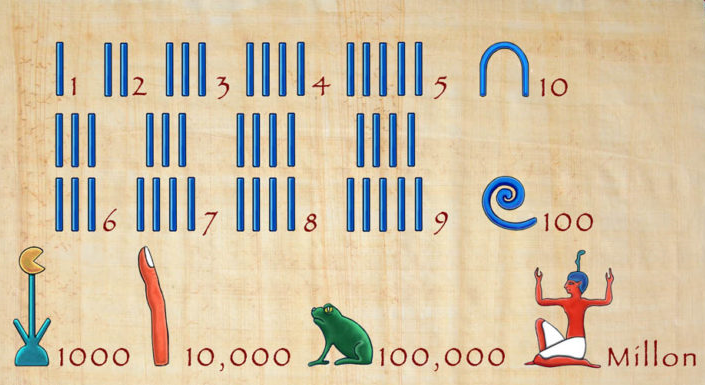
\includegraphics[scale=0.8]{img/hieroglyphic-numbers}
 \caption{Hierogyphic numerals in ancient Egypt.}
 \label{fig:egypt-hieroglyphic-numerals}
\end{figure}

\index{ancient Egypt numerals}
To build the great pyramid, ancient Egyptian created many symbols for big numbers, as shown in \cref{fig:egypt-hieroglyphic-numerals}. They used the symbol of Heh, the god of infinity in Egyptian religion, to represent a million; a tadpole for 100,000; a finger for 10,000; a lotus for a thousand; a rope for a hundred. Repeated grouping when count numbers, if exceeded then grouped to higher level of unit. The value of such a number is the sum of the products of the unit and digit. \Cref{fig:egypt-number-examples} shows two examples.

\begin{figure}[htbp]
 \centering
 \subcaptionbox{212427 is $2(100,000)+1(10,000)+2(1,000)+4(100)+2(10)+7(1)$}{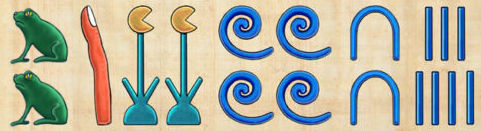
\includegraphics[scale=0.5]{img/egypt-num-eg2}}
 \subcaptionbox{The number, 1,333,330, is inscribed in Edfu temple in Egypt.}{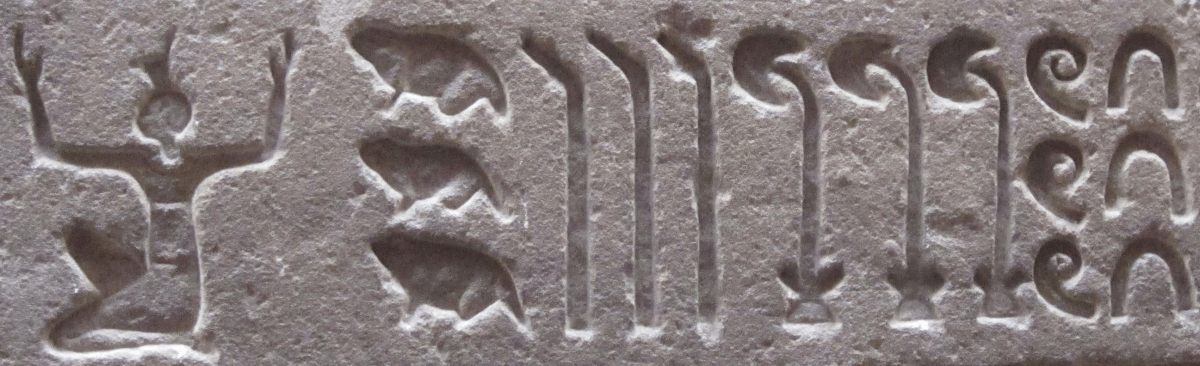
\includegraphics[scale=0.2]{img/Hieroglyphic-num-eg}}
 \caption{Egyptian numbers}
 \label{fig:egypt-number-examples}
\end{figure}

\index{ancient Babylonian numerals} \index{sexagesimal} \index{cuneiform}
Although method (3) can handle big numbers, method (2) is convenient for small numbers. Ancient Babylonians lived in Mesopotamia. The name of the region comes from a Greek word, meaning `between rivers'. It refers to the center of the land between Tigris and Euphrates rivers (in Iraq nowadays). The people impressed their symbols in damp clay tablets. After drying in the sun or in a kiln, the tablets became as permanent as stone. Because the symbol given by the stylus is wedge-shaped, the inscriptions are known as cuneiform\footnote{Combined from `wedge' (cuneus in Latin) and `shape' (forma in Latin).}. Ancient Babylonians used sexagesimal (base 60) system, which is partly left today. For example, a minute has 60 seconds; an hour has 60 minutes. An hour 12 minutes and 30 seconds is written as 1:12:30, which equals $1(60\times 60) + 12(60) + 30 = 4350$ seconds. 60 is not a small number, it appears ancient Babylonians used a mixed system in practical: grouped with 10 for numbers less than 60, otherwise, grouped with $60^2$、$60^3$、$60^4, \dotsc$. \Cref{fig:babylonian-numerals} shows the cuneiform symbols from 1 to 59. We can easily see the pattern: a vertical wedge (Y) for number 1, add such a wedge for each number from 2 to 9; a horizontal wedge (<) for 10, from 11 to 19, the number is a horizontal wedge (10) plus the corresponding vertical wedges. Two horizontal wedges for 20, then repeated the rule within 60, i.e., 10 times the number of horizontal wedges plus the number of vertical wedges.

\begin{figure}[htbp]
 \centering
 \subcaptionbox{Numbers from 1 to 59 in ancient Babylonia.\label{fig:babylonian-numerals}}{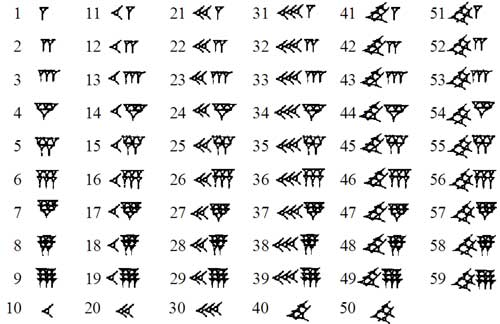
\includegraphics[scale=0.8]{img/Babylonian-numerals}} \\
 \subcaptionbox{Example: $1(60^3) + 19(60^2) + 21(60) + 54$\label{fig:babylonian-num-eg}}{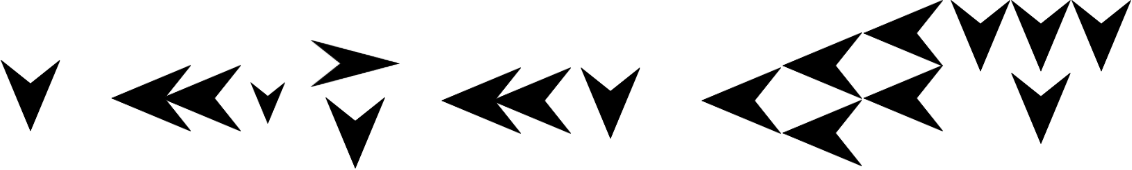
\includegraphics[scale=0.2]{img/Babylonian-num-eg}}
 \caption{Ancient Babylonian numerals.}
\end{figure}

\index{Positional numeral system}
However, numbers greater than 60 have different pattern, as shown in \cref{fig:babylonian-num-eg}. 285714 is 1:19:21:54 in sexagesimal format, but 19 was written as $20 - 1$, where the small vertical wedge means minus. The number being subtracted is annotated with a wedge pointed to right. Evidently, this is not strictly our 60-based number today, but a mixed one with subtraction within 60. Different from Egyptian, ancient Babylonian didn't create dedicated symbols for $60, 60^2, 60^3, \dotsc$; the value of a digit is determined by its position. The left most is the number of 1s, the second is the number of units of 60, the third is the numbe of units of $60^2$, and so on. This is called the positional system. However, ancient Babylonian numbers might have ambiguity because lack of zero. Actually, they invented a symbol for empty place about 300 BCE, but it was used only in the middle of a number but not at the end. As a result, we can't distinguish between 11 and 1100; The later translators suffer from this problem and have to guess from the context.

\section{Roman numerals and Chinese numerals}
\index{Multiplicative grouping system} \index{Roman numerals}

Roman numerals have strong influence still today as the arising of the Roman emperor across Europe, Africa, and Asia. We still see Roman numbers in clocks (see \cref{fig:clock-plate}), buildings, table of content of books. It's easy for memorize as there are only few letters: I, V, X, C, and M. It's convenient to represent small numbers, such as III for 3, VII for 5 (= 2 + 7). 2025 which is MMXXV contains two 1000, two 10, and 5. However, there are so many ways to represent a number, that brings big confusion to decipher. At the beginning, people only needed to sum up the numbers of each letter, but then came the rule of `subtracting on the left and adding on the right'. For example, IV means $5 - 1 = 4$, but VI means $5 + 1 = 6$. Hence IXX $= (10 - 1) + 10 = 19$, while $19 = 10 + (10 - 1) =$ XIX causes ambiguity, because XIX can also be interpreted as (XI)X = 11 + 10 = 21. Similarly, XVIII = 16, but then both $16 = 8 + 8 =$ IIXIIX and $16 = (10 - 4) + 10 =$ IIIIXX have ambiguity. Where IIIIXX for 88 appeared in a Pairs treaty of 1388\cite{LeVeque-Smith-25}.

\btab{|c|c|c|c|c|}
\hline
1 & 5 & 10 & 100 & 1000 \\
\hline
I & V & X  & C   & M \\
\hline
\etab

\begin{figure}[htbp]
 \centering
 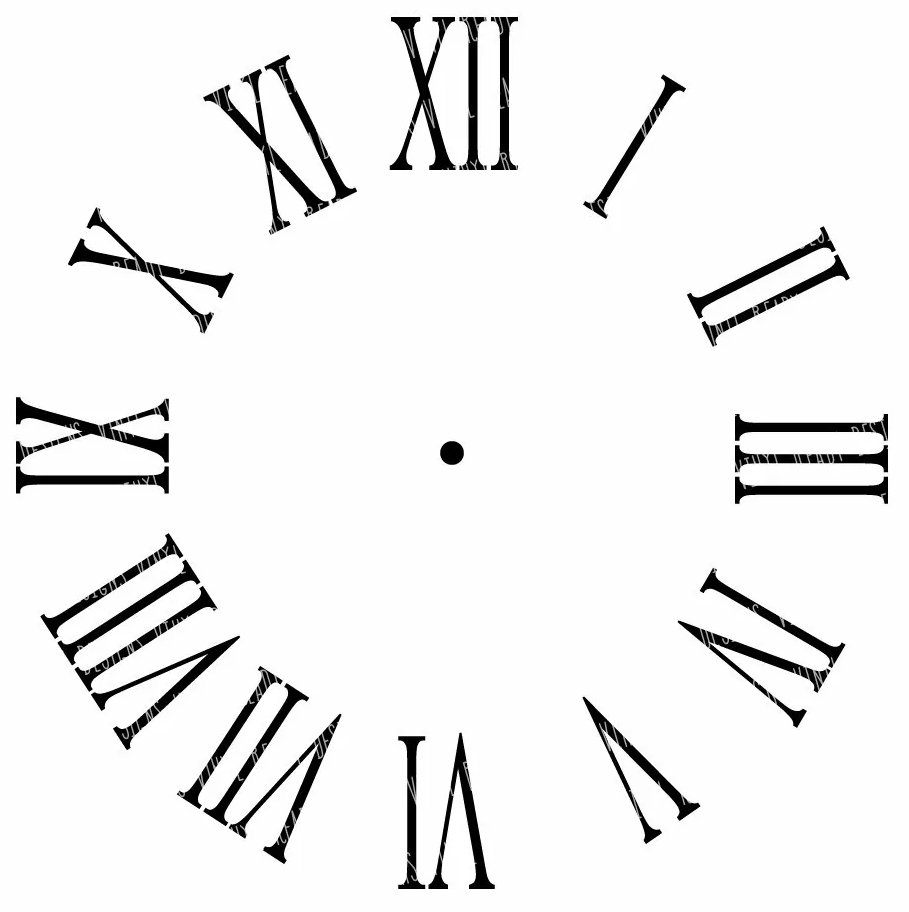
\includegraphics[scale=0.4]{img/clock-plate}
 \caption{Roman numerals in clock plate}
 \label{fig:clock-plate}
\end{figure}

\index{ancient Chinese numerals}
在古代中国产生了非常接近现代计数系统的十进制“乘法分组”计数法。汉字的前10个数字符号是:

\begin{center}
\begin{tabular}{cccccccccc}
一 & 二 & 三 & 四 & 五 & 六 & 七 & 八 & 九 & 十 \\
\end{tabular}
\end{center}

接下来中文没有出现英文中eleven(剩一)和twelve(剩二)的问题,而是直接进展到十一、十二……十九、二十……九十九。数字较小时,也使用廿(20)和卅(30)这样的单位,通常用在日历中。然后增加了百、千、万的分组单位。例如6147写为六千一百四十七,表示6个千、1个百、4个十、7个一,即6千1百4十7个,换成罗马单位相当于6M1C4X7I。每个数字乘以单位的大小,然后加到一起就是数值。这看起来和我们日常生活中的数字几乎一样了,可是几乎毕竟是几乎,究竟还差了一些。比如六千一百七,究竟是6170还是6107?汉字中不是有“零”么?可是在公元十世纪前的古代中国,零从来没有用在数学上。零是一个形声字,雨表形,令表声。本意是下雨。例如《诗经·豳风·东山》:我来自东,零雨其濛。引申意是落下,例如《诗经·郑风·野有蔓草》:野有蔓草,零露漙(tu\'{a}n)兮。《楚辞·离骚》:惟草木之零落兮,恐美人之迟暮。在可能成书于东汉时期的《九章算术》中,没有出现任何含有汉字零的数字。即使在宋元以后引入了零,用法也不一致。例如103可以写成一百零三,也可以写成一百有三。《水浒传》里的好汉数目常读作一百单八将。北京土话中用“二百五”形容一个人愚钝,指的是250。在没有零的情况下,要想避免歧义就必须明确每个数字所代表的单位。这就需要给不同大小的分组单位命名或创造符号。随着数字的增大就需要更多的单位。但数的增加是无限的,而符号的数目是有限的,早晚有用光的时候。下表列出了中文和英文中越来越大的单位名称。

\index{计数单位}
\begin{center}
% for Pinyin tones: \={a}, \'{a}, \v{}, \.{a}
\begin{tabular}{|l|r|l|r|l|r|}
\hline
百            & $100$      & 秭(z\v{i})    & $10^{24}$ &  恒河沙  & $10^{52}$ \\
\hline
千            & $1000$     & 穰(r\'{a}ng)  & $10^{28}$ & 阿僧祗(zh\={i})  & $10^{56}$ \\
\hline
万            & $10000$    & 沟            & $10^{32}$ & 那由他        & $10^{60}$  \\
\hline
亿            & $10^8$     & 涧            & $10^{36}$ &  不可思议      & $10^{64}$ \\
\hline
兆            & $10^{12}$  & 正            & $10^{40}$ &  无量大数      & $10^{68}$ \\
\hline
京            & $10^{16}$  & 载            & $10^{44}$ &               & \\
\hline
垓(g\={a}i)   & $10^{20}$  & 极            & $10^{48}$ &               & \\
\hline
\end{tabular}
\end{center}

可以看到,汉语中这些大单位词汇,有许多来自佛教\cite{Noguchi2007}。包括恒河沙,它表示1后面跟着52个0。英语中的大单位如下表。从一开始,每增加一千倍就有一个对应的单位。万进位和千进位的不同,也是文化上的一种差异。

\begin{center}
\begin{tabular}{|l|r|l|r|l|r|}
\hline
thousand & $10^{3}$ & quattuordecillion & $10^{45}$ & octovigintillion & $10^{87}$ \\
\hline
million & $10^{6}$ & quindecillion & $10^{48}$ & novemvigintillion & $10^{90}$ \\
\hline
billion & $10^{9}$ & sexdecillion & $10^{51}$ & trigintillion & $10^{93}$ \\
\hline
trillion  & $10^{12}$ & septdecillion & $10^{54}$ & untrigintillion & $10^{96}$ \\
\hline
quadrillion  & $10^{15}$ & octodecillion & $10^{57}$ & duotrigintillion & $10^{99}$ \\
\hline
quintillion  & $10^{18}$ & novemdecillion & $10^{60}$ & googol & $10^{100}$ \\
\hline
sexillion    & $10^{21}$ & vigintillion & $10^{63}$ & & \\
\hline
septillion   & $10^{24}$ & unvigintillion & $10^{66}$ & & \\
\hline
octillion    & $10^{27}$ & duovigintillion & $10^{69}$ & & \\
\hline
noniliion  & $10^{30}$ & trevigintillion & $10^{72}$ & & \\
\hline
decillion  & $10^{33}$ & quattuorvigintillion & $10^{75}$ & & \\
\hline
undecillion   & $10^{36}$ & quinvigintillion & $10^{78}$ & & \\
\hline
duodecillion  & $10^{39}$ & sexvigintillion & $10^{81}$ & & \\
\hline
tredecillion  & $10^{42}$ & seprvigintillion & $10^{84}$ & & \\
\hline
\end{tabular}
\end{center}

表中最后一个大单位古格尔(googol)是在1920年由9岁的米尔顿$\cdot$西洛塔(Milton Sirotta)想出的名字。这个数字是1后面跟着100个零。著名的互联网公司谷歌的名字就来自它。

\section{位值制计数系统}
\index{位值制计数系统} \index{玛雅计数系统} \index{太阳年}

在大航海时代,西班牙探险者在中美洲的尤卡坦半岛(位于墨西哥湾和加勒比海之间)发现玛雅文明创造出了完美的计数系统。\cref{fig:maya-numerals}给出了玛雅数字。类似古巴比伦的10-60混合进制,玛雅人使用5-20混合进制。20以内采用5进制,每数1画一个点,每数到5划一横线。20以上的数竖着写,并规范使用0做占位符,如\cref{fig:maya-numerals}所示。玛雅人的计数系统和玛雅历法相互影响。以地球围绕太阳旋转一周作为一个太阳年,每月20天。玛雅人很快发现$20 \times 18 = 360$,接近一年。于是规定1年18个月,在加上5个禁忌日,一年恰好是365天。每4年再加上1天。这和我们现今太阳年的天数几乎一样。

\begin{figure}[htbp]
 \centering
 \subcaptionbox{20以内采用5进制}{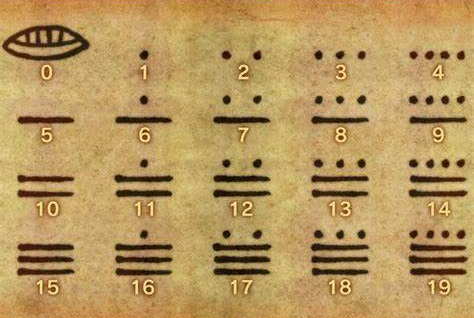
\includegraphics[scale=0.9]{img/Maya-numerals}}
 \subcaptionbox{$2(20^3) + 0(20^2) + 6(20) + 13 = 16133$}{\qquad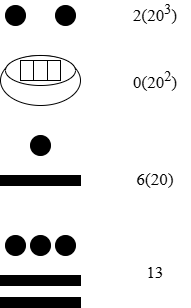
\includegraphics[scale=0.4]{img/Maya-num-eg}\qquad}
 \caption{玛雅数字}
 \label{fig:maya-numerals}
\end{figure}

无论是玛雅的20进制还是古巴比伦的60进制,都不需要额外命名单位,而是通过数字所在位置赋予大小的意义。这种方法叫做位值制计数系统(positional numeral system),归纳起来有3个要求:

\begin{enumerate}[1)]
\item 确定一个进制\footnote{英文base的首字母}$b$。如我们日常使用的$b = 10$、古巴比伦使用的$b = 60$、玛雅使用的$b = 20$。
\item 给1、2……$b-1$这些数字命名。例如汉语的一、二、三……九;英语的one, two, three, ..., nine;玛雅的点、点点……四点三划。
\item 代表0的符号。
\end{enumerate}

这样任何一个数$n$等于:

\be
n = a_m b^m + a_{m-1} b^{m-1} + \cdots + a_a b + a_0
\label{eq:pos-rep}
\ee

其中$a_i$是被命名的数字,包括0、1、2……$b-1$。$n$写为$a_ma_{m-1} \cdots a_0$。例如$2024 = 2 \times 10^3 + 0 \times 10^2 + 2 \times 10 + 4$, 其中$b = 10, m = 3, a_3 = 2, a_2 = 0, a_1 = 2, a_0 = 4$,恰好也写为2024。注意0在这里起到了关键的“占位”作用——总共有2个千、2个十、4个一,但是没有百。0占据在百的位置上,这样其它数字才能“各就各位”,避免出现224这样的问题。我们再看一正一反两个例子:

\begin{example}
猫咪王国中,每只猫爪只有4个可动的指(见\cref{fig:cat-paw}),左右共8个可动的指。如果采用8进制,并规定0的符号为“喵”,1到7为:(1)苗、(2)秒、(3)妙、(4)咪、(5)谜、(6)米、(7)蜜。王国一年的天数$365 = 5 \times 64 + 5 \times 8 + 5$,写成“谜谜谜”。$2024 = 5 \times 8^3 + 3 \times 8^2 + 7 \times 8 + 0$,写成“谜妙蜜喵”。

\begin{figure}[htbp]
 \centering
 
\includegraphics[scale=0.6]{img/cat-paw}
 \caption{猫爪}
 \label{fig:cat-paw}
\end{figure}

\end{example}

\begin{example}
\index{干支纪年}
\textbf{反例:}我国古代用天干地支纪年。天干有10个符号:甲、乙、丙、丁、戊、己、庚、辛、壬、癸;地支有12个符号:子、丑、寅、卯、辰、巳、午、未、申、酉、戌、亥。组合起来可以记录60以内的数字,从甲子开始,接下来天干地支各向前进一到已丑,然后是丙寅……到癸亥结束(见\cref{fig:sexagenary})。比如2025年是农历乙巳年。乙的上一个天干符号是甲,巳的上一个地支符号是辰,所以前一年2024年是甲辰年,后一年2026年是丙午年。尽管我们不说“丙天午地”,看似用位置表示(第一个符号是天干、第二个符号是地支),但干支纪年{\em 不是位值制计数法}。例如丙午并非一个甲子中的第$3 \times 10 + 7 = 37$年,而是第43年\footnote{除了查看\cref{fig:sexagenary}外,也可以这样计算:天干每10年循环,地支每12年循环。丙是天干中的第3个符号,午是地支中的第7个符号,所以丙午年除以10余3且除以12余7。60中除以10余3的数字有3、13……43、53,其中只有43除以12余7。}。

\begin{figure}[htbp]
 \centering
 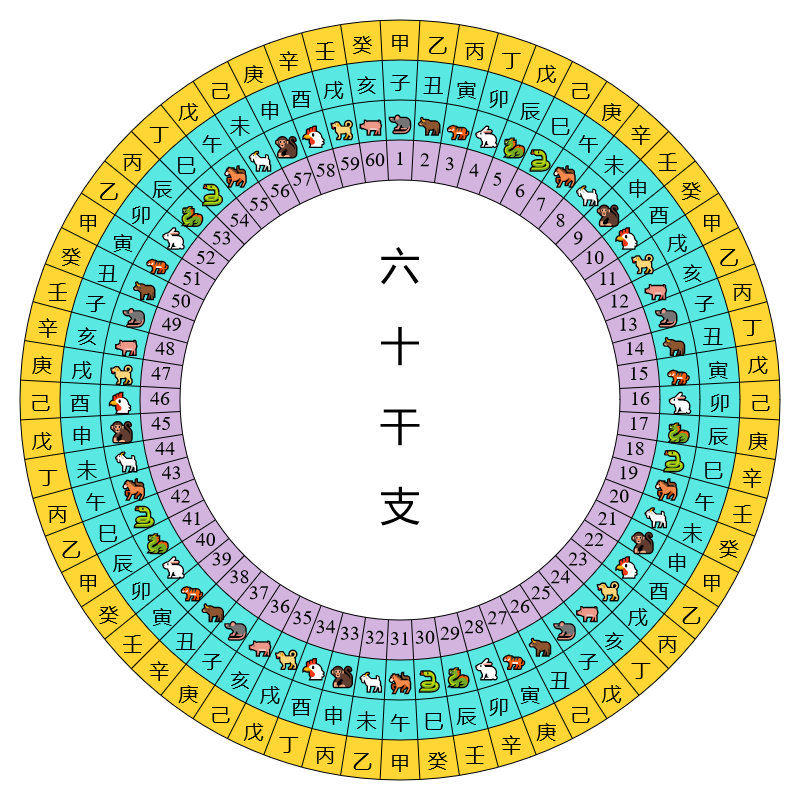
\includegraphics[scale=0.3]{img/sexagenary-chinese}
 \caption{干支纪年}
 \label{fig:sexagenary}
\end{figure}

\end{example}

罗马数字的一个问题就是歧义——一个数字有多种写法或一个写法可以代表不同的数字。位值制能解决这个问题么?明显8 = 08 = 008。我们在电梯、数字钟,汽车里程表上都见过类似的情况。可以在一个数字前放任意多个零而不改变值。如果对最高位的数字加以限制,规定\cref{eq:pos-rep}中的$a_m \neq 0$,那么一个数的位值制表示是唯一的(见\cref{qn:unique-pos-rep})。

% (1) Brahmi, 1st Century CE, (2) Indian (Gwalior), 9th Century, (3) Sanskrit Davanagari, Indian, 11th Cenntury, (4) West Arabic (Gubar? Gobar?), 11th Century, (5) East Arabic, 11th Centry, (still used in Turkey), (6) 15th Century, (7) 16th Century (Dürer)
\begin{figure}[htbp]
 \centering
 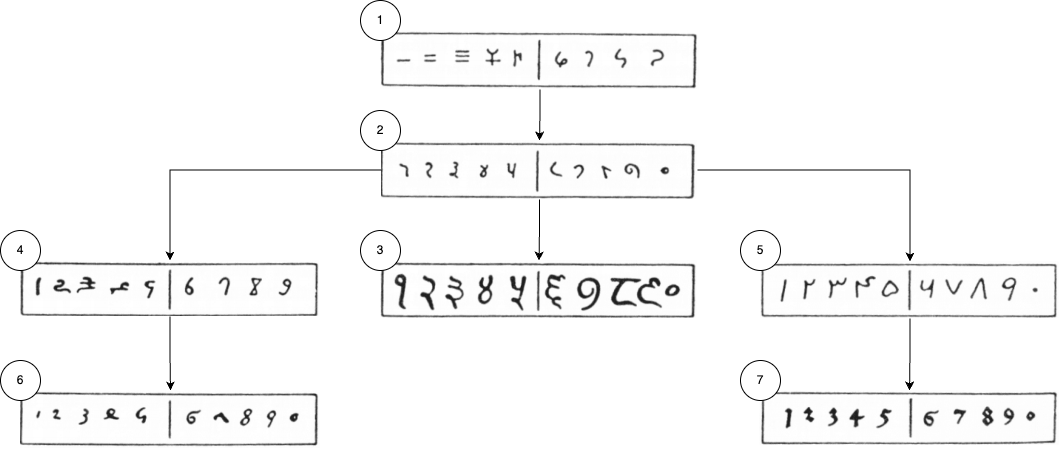
\includegraphics[scale=0.3]{img/Hindu-arabic-num}
 \caption{印度——阿拉伯数字的演进:1、婆罗门数字,公元一世纪;2、印度瓜廖尔数字包括0,公元九世纪;3、4、5、梵文天成体、东、西阿拉伯数字,公元十一世纪,其中西阿拉伯数字至今仍在土耳其使用;6、7、十五和十六世纪。}
 \label{fig:hindu-arabic-numerals}
\end{figure}

\index{印度——阿拉伯计数系统} \index{零} \index{数学家!婆罗摩笈多} \label{sec:hindu-arabic-numerals}
在历史的长河中,玛雅人和古巴比伦人的计数系统都湮没了。20和60以内的数字并非单一符号,混合进制难于计算。现代位值制系统是印度文明发展出并经由阿拉伯人传入西方的,被称作“印度——阿拉伯系统”(Hindu-Arabic system)。在公元前三世纪,印度的碑铭中出现了1、4、6这样的符号;在公元一、二世纪的岩洞中,形如2、3、4、5、6、7、9的符号也出现了。可以看出2从二、3从三中演化的迹象,在公元七世纪,印度数学家婆罗摩笈多定义了零\cite{MacTutor-Brahmagupta-2000}。但直到公元九世纪以前,符号0仍未出现(见\cref{fig:hindu-arabic-numerals})。印度人首先用一个点或小圆圈表示零,命名为sunya,梵文的意思是“空位”。传入阿拉伯后译为sifr,意思是“保持完整”。1140年,它伴随着阿拉伯学者花拉子密的著作被音译为拉丁文,最后变为今天英语中的zero。

\begin{mdframed}

\begin{center}
 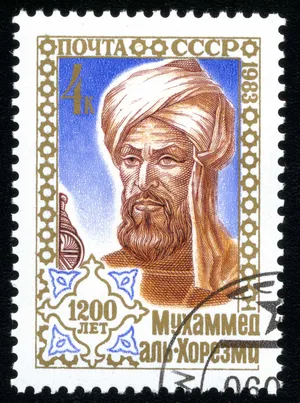
\includegraphics[scale=0.3]{img/Khwarizmi}
 \captionof{figure}{前苏联1983年发行的花拉子密纪念邮票}
 \label{fig:kwarizmi}
\end{center}

\index{数学家!花拉子密} \label{sec:Khwarizmi}
公元七世纪初,阿拉伯文明崛起。罗马帝国分裂后,古希腊、拜占庭、印度的数学成果逐渐在八世纪汇集到阿拉伯帝国。阿拔斯王朝于公元830年在巴格达设立了著名的“智慧宫”,聚集了大批学者研究整理来自世界各地的天文地理资料和学术成果。公元813年,著名学者阿尔·花拉子密(al-Khwārizmī,约780~约850,见\cref{fig:kwarizmi})来到巴格达,并成为智慧宫的主要学者之一。关于花拉子密的生平,我们知之甚少。甚至他的名字可能只是个“绰号”。阿拉伯文al是“来自”的意思,Khwārizmī是地名“花剌子模”,位于今天中亚的乌兹别克斯坦境内。金庸先生的小说《射雕英雄传》中有黄蓉帮着成吉思汗用计攻下花剌子模的故事,说的就是这个地方。花拉子密在数学方面完成了两部传世之作:《代数学》(成书于820年)和《印度数字算术》(成书于825年)。此外他还完成了地理和天文方面的著作。《代数学》的拉丁文译名为Hisab al-jabr w'al-muqabala,意思是还原与对消的科学。其中al-jabr后来演变为英文algebra。1859年清代学者李善兰与传教士伟烈亚力创造性地把它译为中文“代数”\cite{HanXueTao2009}。花拉子密在书中系统地给出了一元一次、二次方程的代数解法。但是他所在的时代还没有代数符号系统,因此完全使用文字来描述问题和解题步骤,并附加上几何解释来说明正确性。《印度数字算术》在十二世纪被翻译为拉丁文(Liber Algorismi de numero Indorum)并传入欧洲,促进了印度——阿拉伯十进制计数系统的传播。花拉子密名字的拉丁音译Algorismi后来成了“算法”一词Algorithm\cite{Britannica-25}。

%% https://www.britannica.com/print/article/317171
%% https://mathshistory.st-andrews.ac.uk/Biographies/Al-Khwarizmi/
\end{mdframed}

十进制位值制系统带来了巨大优势,便于计算并可以处理任意大的数字。我们可以想象用罗马数字计算MMXXV - CXXXVII有多么困难,而小学生也可以用竖式快速算出结果:

\begin{center}
\opsub[voperator=bottom]{2025}{137}
\end{center}

\label{sec:counting-rods} \index{算筹}
这仅仅是减法,更不用说乘除法了。尽管古汉语中的计数系统并非位值制(见上一节),古代中国却发展出了一套严格意义上的位值制计算方法——筹算。筹算使用若干小棍进行计算。这些小棍用竹子制成叫做算筹\footnote{形声字“筹”的形旁是竹。也有用木头、兽骨、象牙、金属等材料的。}。它的发明是一个漫长的过程,但春秋战国时期已经普遍使用了。成语“运筹帷幄”、“一筹莫展”、“技高一筹”都反映了算筹的使用情况。算筹有横竖两种摆法,如\cref{fig:suanchou-digit}所示。如果个位竖着摆,则十位横着摆。这样交错摆放避免混淆。如果某一位是零,则空出不摆放\footnote{在计算过程中空位可能不明显造成混淆。后来人们在书写记录算筹运算结果时,就在应该是零的数位上写 “$\square$” 或 “〇”。}。算筹进行竖式计算非常方便,尤其是处理进位和借位。例如进位时只要把一个小棍摆到下一位就可以了。如\cref{fig:suanchou-eg}所示。

\begin{figure}[htbp]
 \centering
 \subcaptionbox{算筹数字的横竖摆法 \label{fig:suanchou-digit}}{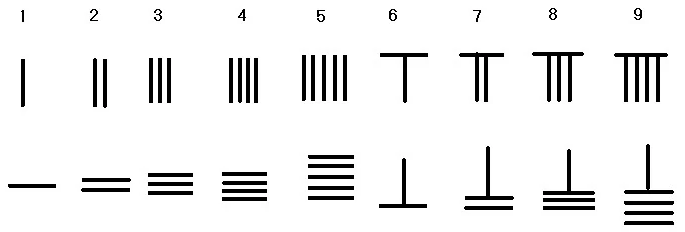
\includegraphics[scale=0.25]{img/suanchou-digit}}
 \subcaptionbox{算筹计算2025 - 137 \label{fig:suanchou-eg}}{\qquad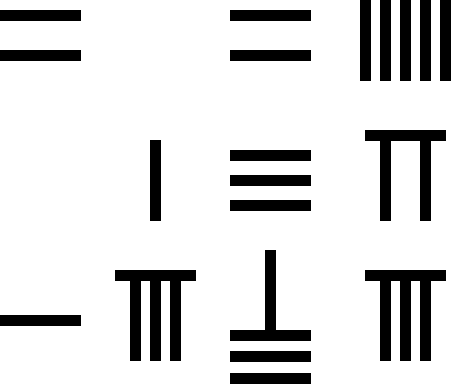
\includegraphics[scale=0.15]{img/suanchou-eg}\qquad}
 \caption{算筹}
\end{figure}

\index{数学家!斐波那契}
花拉子密的著作一开始只有少数学者了解。1202年斐波那契通过他的著作《算盘书》(Liber Abaci)进一步把印度——阿拉伯系统和计算方法介绍到欧洲。无独有偶,“斐波那契”其实也是个绰号。这位中世纪的数学家叫列奥纳多,来自比萨,所以称作比萨的列奥纳多。斐波那契来自拉丁文filius Bonacci,意思是波那契之子。斐波那契的父亲当时是商人,在北非以及地中海一带经商。斐波那契逐渐从埃及人、希腊人、西西里人、阿拉伯人那里学到了各种数字系统。他逐渐认识到了印度——阿拉伯数字的先进性。《算盘书》不仅包括位值制的记法,还讲解了如何计算利润率、利息、汇率、度量衡换算等实际问题。一经面试大受欢迎,被广泛传抄。神圣罗马帝国皇帝腓特烈二世听说了斐波那契,在1225年邀请他到比萨。斐波那契接受了宫廷数学家的挑战,成功解决了所有题目,包括一道一元三次方程。他采用的数值解法给出了9位小数精度\cite{Gies-Carney-24}。今天,以他命名的“斐波那契数列”,即1、1、2、3、5、8……已经家喻户晓。我们将在第\ref{sec:Fibonacci-numbers}节详细介绍这个有趣的数列。

\begin{figure}[htbp]
 \centering
 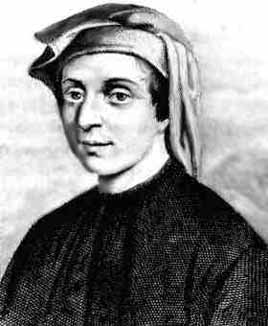
\includegraphics[scale=0.35]{img/Fibonacci}
 \caption{比萨的列奥纳多(斐波那契)1175-1250}
 \label{fig:Fibonacci}
\end{figure}

\label{sec:binary-numerals} \index{二进制}
越来越多的学者和在各国往来贸易的商人把印度——阿拉伯计数系统传播到了全球。它成了全人类的通用语言。十七世纪时,德国数学家莱布尼茨提出了二进制,它导致了计数系统在二十世纪产生了革命性的应用。电子计算机内部使用二进制对数字和信息编码。尽管二进制只有0、1两种数字,表示很长,例如2025写成二进制是1111 1101 001,但0、1两种状态可以通过电路的通、断或电平(电压)的高、低方便地实现。还有一个好处:0、1可以对应逻辑的真、假;事物的有、无;答案的对、错,从而方便用机器统一处理数和逻辑,如\cref{tab:binary-arithmatic-logic}。

\begin{table}
\[\begin{array}{cccc}
  \begin{tabular}{c|c}
  $x$ & $1-x$ \\
  \hline
  0 & 1   \\
  \hline
  1 & 0   \\
  \end{tabular}
  &
  \begin{tabular}{c|c}
  $x$ & 非 $x$ \\
  \hline
  假 & 真  \\
  \hline
  真 & 假   \\
  \end{tabular}
   \quad & \quad
  \begin{tabular}{c|c|c}
  $x$ & $y$ & $x \times y$ \\
  \hline
  0 & 0 & 0  \\
  \hline
  0 & 1 & 0  \\
  \hline
  1 & 0 & 0  \\
  \hline
  1 & 1 & 1  \\
  \end{tabular}
  &
  \begin{tabular}{c|c|c}
  $x$ & $y$ & $x$ \text{与} $y$ \\
  \hline
  假 & 假 & 假 \\
  \hline
  假 & 真 & 假 \\
  \hline
  真 & 假 & 假 \\
  \hline
  真 & 真 & 真 \\
  \end{tabular}
\end{array}\]
\captionof{figure}{二进制$1-x$与逻辑非的对应、乘法和逻辑与的对应}
\label[figure]{tab:binary-arithmatic-logic}
\end{table}

我们的祖先从狩猎、采集、计数开始,经过了四千余年才发展出了现代十进制位值制计数系统。数的诞生实在是一个漫长曲折的过程。它没有一个确定的发明者,而是在各个文明中独立产生于生产劳动,互相影响,逐渐发展,是人类群体性的进步。

\begin{Exercise}[label={ex:numerals}]
\Question{2025年深圳市南山区小学4年级期末数学考试中出现了这样一道题:“计算$114 \times 21$,同学们用了不同的方法。在思路上这些方法有什么相同的地方?”

\begin{multicols}{2}
\begin{enumerate}
  \renewcommand{\labelenumi}{\textcircled{\theenumi}}
  \item
    \begin{align*}
      114 \times 20 & = 2280 \\
      114 \times 1  & = 114 \\
      2280 + 114 & = 2394
    \end{align*}

  \item
    \begin{align*}
       & 114 \times 21 \\
     = & 114 \times 7 \times 3 \\
     = & 798 \times 3 \\
     = & 2394
    \end{align*}

  \item
    \[\begin{array}{cc}
    \begin{tabular}{|c|c|c|c|}
      \hline
      \times & 100  & 10  & 4 \\
      \hline
      20       & 2000 & 200 & 80 \\
      \hline
      1        & 100  & 10  & 4 \\
      \hline
    \end{tabular}  \quad
    \opadd[voperation=center,
           voperator=bottom]{2280}{114}
    \end{array}\]

  \item
    \opmul[displayshiftintermediary=all,
           voperator=bottom,
           voperation=top]{114}{21}
    \oplput(1,-2){$\cdots$ \opmul[style=text]{114}{1}}
    \oplput(1,-3){$\cdots$ \opmul[style=text]{114}{20}}
\end{enumerate}
\end{multicols}
这四个方法中,哪些利用了十进制位值制计数系统的优势?
}

\Question{可以利用$n = a_m b^m + a_{m-1} b^{m-1} + \cdots + a_a b + a_0$进行进制转换:
  \begin{enumerate}[1)]
    \item 用$n$除以$b$得到余数$a_0$、商$q_0$。
    \item 把$n$替换为$q_0$,再次用$n$除以$b$得到余数$a_1$、商$q_1$。
    \item 把$n$替换为$q_1$,重复上述步骤直到商$q_m = 0$。
  \end{enumerate}
  则$n$的$b$进制表示为$a_m \cdots a_1a_0$。请将十进制数123转换为(a)玛雅文;(b)古巴比伦文;(c)计算机二进制表示。
}

\Question{$\bigstar$\footnote{标星号的题目较难。}如果你会编程,请用自己熟悉的语言实现二进制到十进制的相互转换。}

\Question{$\bigstar$证明一个数的位值制表示是唯一的。提示:考虑如果一个数有两种表示会怎样? \label{qn:unique-pos-rep}}
\end{Exercise}

\begin{Answer}[ref={ex:numerals}]
\Question{ \textcircled{1}、\textcircled{3}、\textcircled{4} }

\Question{将十进制数123转换为(a)玛雅文;(b)古巴比伦文;(c)计算机二进制表示。

玛雅文:

\begin{align*}
123 \div 20 &= 6 \cdots 3 & \underline{\ \circ \ } \\
6 \div 20 &= 0 \cdots 6   & \circ \circ \circ \\
120 &= 6 (20) + 3  &  \text{从上到下6、3}
\end{align*}

古巴比伦文:YY YYY
\begin{align*}
123 \div 60 &= 2 \cdots 3 \\
2 \div 20 &= 0 \cdots 2   \\
120 &= 2 (60) + 3
\end{align*}

计算机二进制表示:1111011
\begin{align*}
123 \div 2 &= 61 \cdots 1 &
61 \div 2 &= 30 \cdots 1   &
30 \div 2 &= 15 \cdots 0 \\
15 \div 2 &= 7 \cdots 1 &
7 \div 2 &= 3 \cdots 1 &
3 \div 2 &= 1 \cdots 1 \\
1 \div 2 &= 0 \cdots 1 & & & &
\end{align*}
}

\Question{编程实现二进制到十进制的相互转换。

\begin{center}
 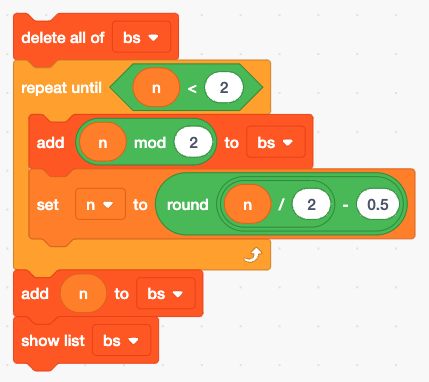
\includegraphics[scale=0.3]{img/scratch-bin}
 \qquad
 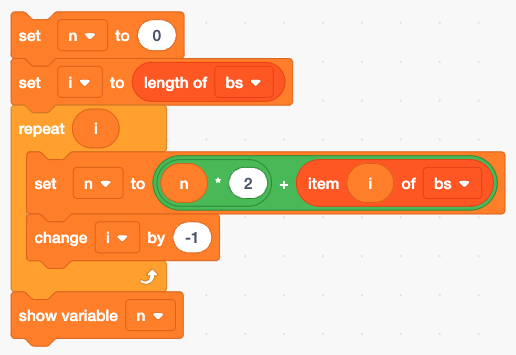
\includegraphics[scale=0.3]{img/scratch-dec}
 \captionof{figure}{Scratch例子程序:十进制$n$与二进制$bs$相互转换,左:$10 \to 2$;右:$2 \to 10$}
 \label{fig:bin-dec-scratch}
\end{center}

说明:\lstinline|round|是四舍五入。对$n/2$ - 0.5四舍五入相当于对$n/2$取整,求得$n$除以2的除数。$bs$中的二进制数字低位在前,高位在后。下面是对应的Python例子程序:

\begin{lstlisting}[language=Python, frame=single]
def bin(n):
    bs = []
    while n > 1:
        bs = [n % 2] + bs
        n = n // 2
    return [n] + bs

def dec(bs):
    n = 0
    for b in bs:
        n = n*2 + b
    return n
\end{lstlisting}

与Scratch和Python的循环不同,下面的Haskell例子给出了递归实现。其中的二进制数字高位在前、低位在后。

\begin{Haskell}[frame=single]
bin x = if x < 2 then [x] else (bin (x `div` 2)) ++ [x `mod` 2]
dec = foldl (\n x -> n*2 + x) 0
\end{Haskell}
}

\Question{证明一个数的位值制表示是唯一的。

\begin{proof}
假设一个数还有另一个表示。如果它们的位数不同,我们在较短的前面添加0,使它们一样长。令补0后的表示分别为$a_{m} a_{m-1} \cdots a_1 a_0$和$c_m c_{m-1} \cdots c_1 c_0$。按照\cref{eq:pos-rep}计算的值相等,即:
\[
  a_m b^m + a_{m-1} b^{m-1} + \cdots + a_1 b + a_0 = c_m b^m + c_{m-1} b^{m-1} + \cdots + c_1 b + c_0
\]

将$a_0$和$c_0$移到右边,剩下的移到左边:

\[
  (a_m - c_m) b^m + (a_{m-1} - c_{m-1}) b^{m-1} + \cdots + (a_1 - c_1) b = c_0 - a_0
\]

左边可以被$b$整除,所以$c_0 - a_0$也可以被$b$整除。由于$c_0$、$a_0$都只能是0到$b - 1$的整数,所以它们的差只能是$1 - b, \dots , -1, 0, 1, \dots b - 1$中的一个。但其中只有0能被$b$整除。所以$c_0 - a_0 = 0$,即$c_0 = a_0$。

接下来$(a_m - c_m) b^m + (a_{m-1} - c_{m-1}) b^{m-1} + \cdots + (a_1 - c_1) b = 0$。由于$b \neq 0$,两边除以$b$,然后将$a_1$和$c_1$移动到左边:

\[
  (a_m - c_m) b^m + (a_{m-1} - c_{m-1}) b^{m-1} + \cdots + (a_2 - c_2) b = c_1 - a_1
\]

同样可以推出$c_1 = a_1$。重复这个步骤$m$次,最后得到$a_m = c_m$。这就证明了两种表示是一样的,即位值制表示是唯一的。
\end{proof}
}
\end{Answer}

\ifx\wholebook\relax \else
\section{Answer}
\shipoutAnswer

\section{Greek alphabet} \label{ch:greek-letters}
\subimport{inc/}{greek-zh-cn}


 \begin{table}[htbp]
     \centering
     \begin{tabular}{|c|c|c||c|c|c|}
         \hline
               \textbf{Upper} & \textbf{Lower} & \textbf{Pronunciation} & \textbf{Upper} & \textbf{Lower} & \textbf{Pronunciation} \\
         \hline
         A         & $\alpha$    & Alpha &      N         & $\nu$         & Nu \\
         B         & $\beta$     & Beta &       $\Xi$         & $\xi$         & Xi \\
         $\Gamma$  & $\gamma$    & Gamma &      O    & o    & Omicron \\
         $\Delta$  & $\delta$    & Delta &      $\Pi$         & $\pi$         & Pi \\
         E         & $\epsilon$  & Epsilon &    P        & $\rho$        & Rho \\
         Z         & $\zeta$     & Zeta &       $\Sigma$      & $\sigma$      & Sigma \\
         H         & $\eta$      & Eta &        T        & $\tau$        & Tau \\
         $\Theta$  & $\theta$    & Theta &      Y    & $\upsilon$    & Upsilon \\
         I         & $\iota$     & Iota &       $\Phi$        & $\phi$        & Phi \\
         K         & $\kappa$    & Kappa &      X        & $\chi$        & Chi \\
         $\Lambda$ & $\lambda$   & Lambda &     $\Psi$        & $\psi$        & Psi \\
         M         & $\mu$       & Mu &         $\Omega$      & $\omega$      & Omega \\
         \hline
     \end{tabular}
     \caption{Greek alphabet}
     \label{tab:greek-alphabet}
 \end{table}

\begin{thebibliography}{99}
\subimport{inc/}{bib-zh-cn}
\end{thebibliography}

\expandafter\enddocument
\fi
